\documentclass{article}

\title{Metodi Numerici per l'Informatica}
\author{Anthony}
\date{02 mag 2023}

\usepackage{amssymb}
\usepackage{amsmath}
\usepackage{graphicx}

\begin{document}
    \maketitle
    \section{Discesa del gradiente: introduzione}
        Abbiamo già affrontato diversi problemi di minimizzazione. È giunta l'ora di chiederci se esiste una 
        ricetta generale per risolvere problemi della forma:
            \[\min_\mathbf{x} f(\mathbf{x}) \]
        In cui $f$ è differenziabile. \\
        La discesa del gradiente è un algoritmo di minimizzazione del \emph{primo ordine}. Ciò significa che 
        utilizza solo le informazioni di primo ordine della funzione, ovvero il suo gradiente, per determinare 
        la direzione e l'ampiezza di spostamento delle variabili; esso non tiene conto di informazioni 
        di ordine superiore, come le derivate seconde. \\
        L'idea generale del gradiente è quella di muoverci dove la funzione scende più velocemente. Quindi, dato un 
        punto di partenza $\mathbf{x}^{(0)}$, computiamo iterativamente il gradiente:
            \[\mathbf{x}^{t+1} = \mathbf{x}^{(t)} - \alpha \nabla f(\mathbf{x}^{(t)})\]
        E ci fermiamo quando raggiungiamo il minimo. 
        Osserviamo ora una funzione $f : \mathbb{R}^2 \mapsto \mathbb{R}$:
        \begin{center}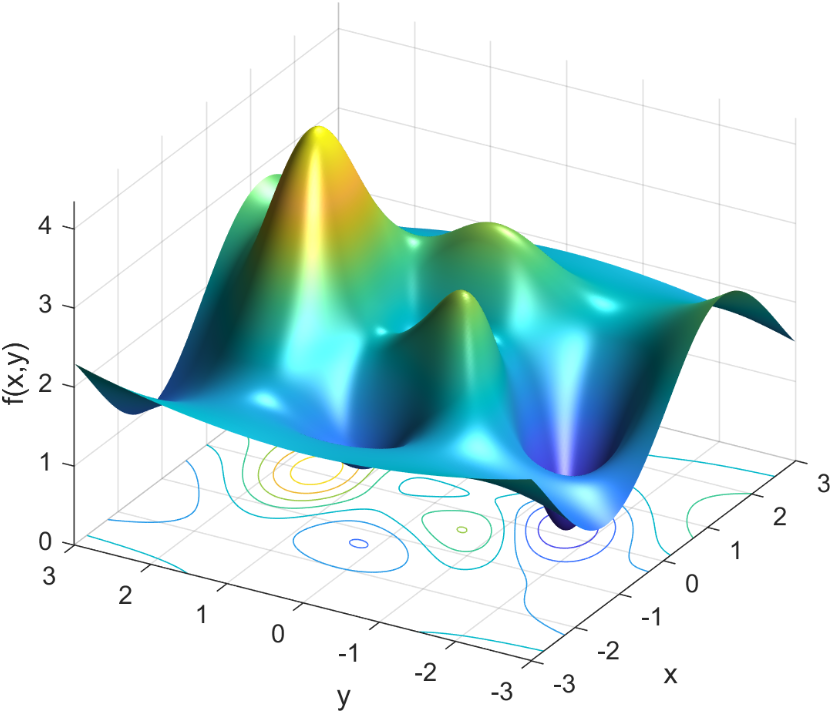
\includegraphics[width=7cm]{funr2.png}\end{center}
        Possiamo rappresentare tale funzione guardando solo le sue $\emph{curve di livello}$ (o isocurve, isocontorni, level set). Le isocurve 
        a tre dimensioni vengono chiamate isosuperfici. Esse 
        rappresentano gli infiniti punti del dominio in cui la funzione ha esattamente lo stesso valore. Le curve di livello, in questo 
        esempio, sono colorate in funzione del loro valore. Osserviamo una porzione di funzione attraverso alcune delle sue curve di livello:
        \begin{center}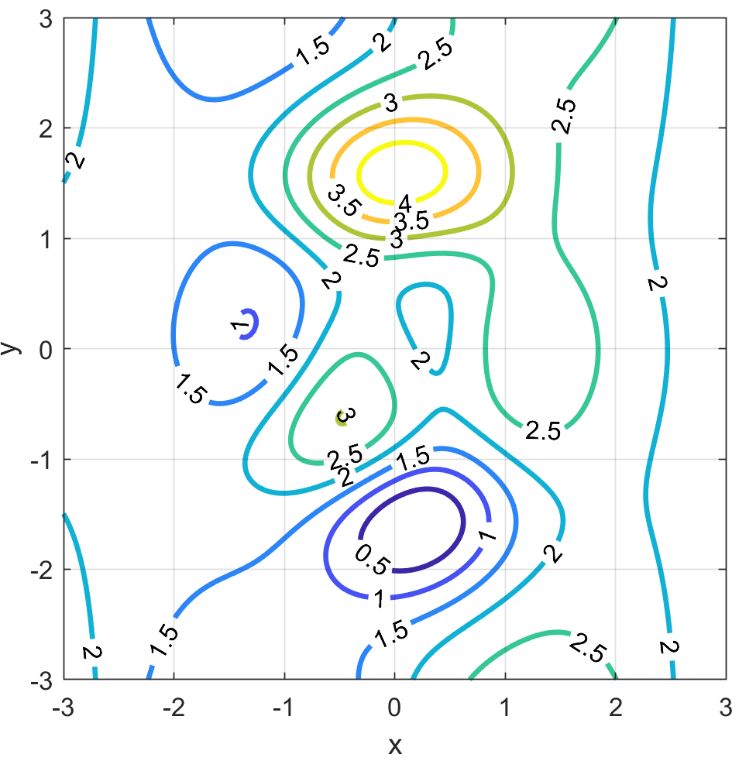
\includegraphics[width=7cm]{curve_livello.png}\end{center}
        Abbiamo già osservato precedentemente che possiamo rappresentare il gradiente come delle frecce sul piano. In particolare 
        rappresentiamo il gradiente negativo di una porzione della nostra funzione esempio:
        \begin{center}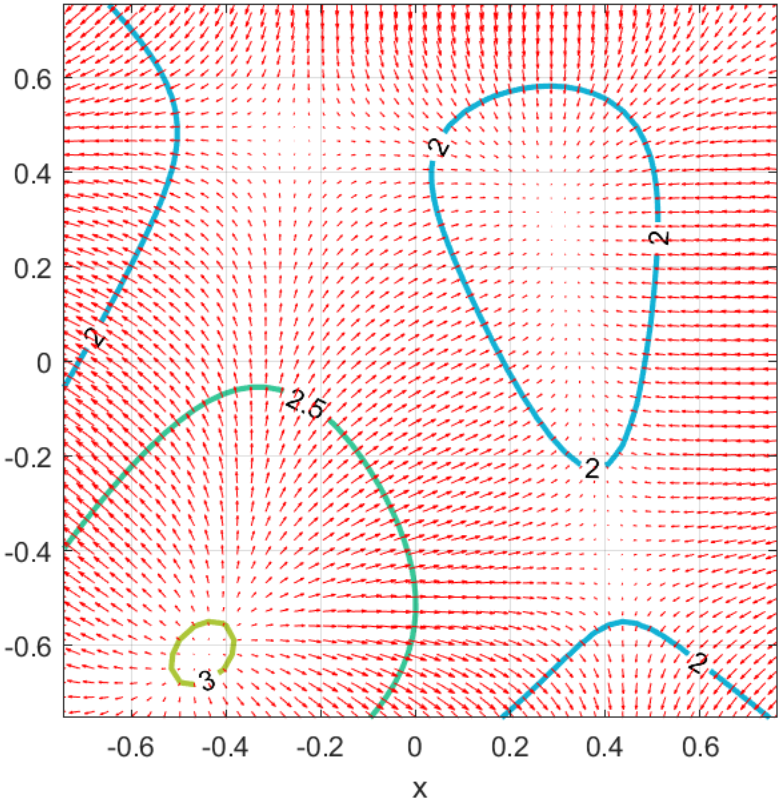
\includegraphics[width=7cm]{neg_grad.png}\end{center}
        Possiamo osservare alcune proprietà:
        \begin{enumerate}
            \item Il gradiente è smooth; questo accade perché la funzione è continua.
            \item Le frecce del gradiente hanno lunghezze diverse, questo perché il gradiente non ha norma unitaria.
            \item Il gradiente, su alcuni punti, sembra assumere una struttura puntiforme e quindi equivale a zero; questi 
            punti rappresentano i minimi locali della funzione.
        \end{enumerate}
        Poiché sono presenti più minimi locali, il criterio di minimizzare il gradiente della funzione pari a zero non è 
        del tutto fattibile, questo perché potremmo arrivare a punti di sella della funzione.
        La discesa del gradiente è un algoritmo generico, ma non dà garanzie sul minimo globale, tuttavia se la funzione è
        convessa, la discesa del gradiente ci garantisce un minimo globale.

    \section{Discesa del gradiente: ortogonalità}
        Possiamo osservare un dettaglio importante: il gradiente è ortogonale rispetto alle curve di livello: supponiamo 
        di piazzarci su una curva di livello e guardiamo in una direzione tangente a essa:
        \begin{center}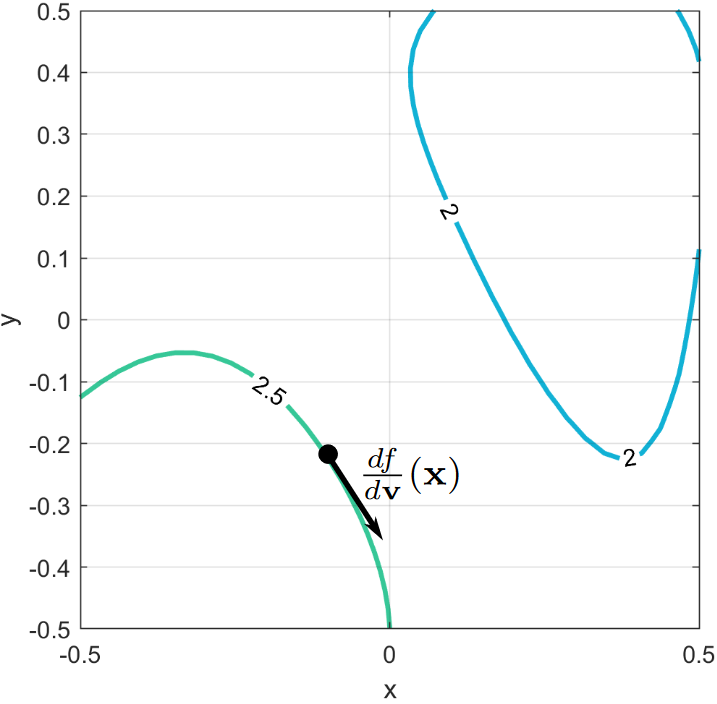
\includegraphics[width=7cm]{grad_orthogonal.png}\end{center}
        Se effettuiamo un passo infinitesimo, otteniamo un nuovo punto in cui la funzione è come prima. Possiamo osservare 
        che la derivata direzionale di $f$ rispetto a un punto generico $\mathbf{v}$ è calcolabile con il prodotto interno tra il 
        gradiente di $f$ e v:
        \[\frac{\partial f}{\partial \mathbf{v}} = \langle \nabla f, \mathbf{v}\rangle \]
        Su un isocurva, la derivata in direzione tangente all'isocurva, è pari a zero. Ciò significa che il prodotto interno 
        tra il gradiente e $\mathbf{v}$ è pari a zero:
        \[\frac{\partial f}{\partial \mathbf{v}} = \langle \nabla f, \mathbf{v}\rangle = 0 \quad \text{quando $\mathbf{v}$ è tangente a un isocurva}\]
        Ciò significa che i due vettori sono ortogonali: il gradiente è quindi 
        ortogonale alle curve di livello. \\

    \section{Discesa del gradiente: differenziabilità}
        L'algoritmo della discesa del gradiente richiede che la funzione $f$ sia differenziabile, ovvero deve avere un 
        gradiente \emph{continuo}, senza spigoli o cambiamenti di segno improvvisi.

    \section{Discesa del gradiente: punti stazionari}
        Definiamo come \emph{punti stazionari} quei punti in cui il gradiente tende a zero. La discesa del gradiente 
        converge nei punti stazionari e non necessariamente si trattano di minimi locali, ma anche punti di sella:
        \begin{center}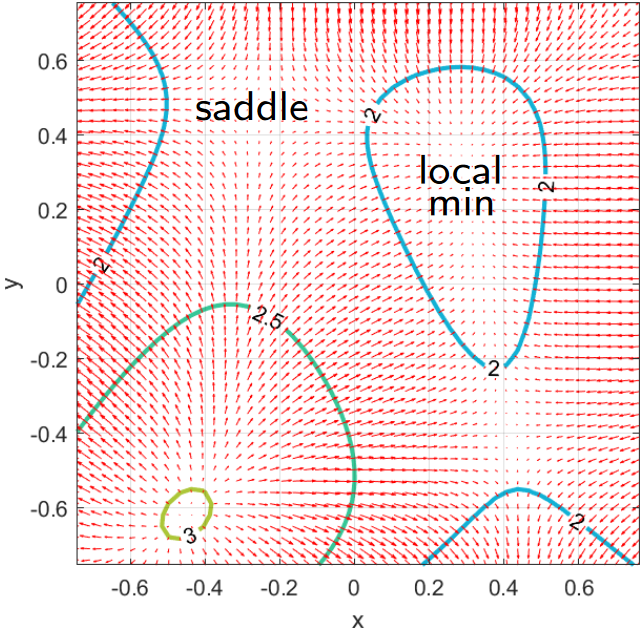
\includegraphics[width=7cm]{stationary_points.png}\end{center}
        \[\mathbf{x}^{t+1} = \mathbf{x}^{(t)} - \underbrace{\alpha \nabla f(\mathbf{x}^{(t)})}_{\text{punto staz.}} = \mathbf{x}^{(t)}\]
        Il risultato finale della discesa del gradiente dipende molto dal punto di inizializzazione. Possiamo osservare che 
        il parametro $\alpha$ influenza la lunghezza del passo. Se scegliamo un 
        $\alpha$ troppo piccolo, procediamo poco alla volta verso il minimo ma ci vorranno tante direzioni. Se invece 
        $\alpha$ è troppo grande, potremmo non raggiungere mai la convergenza. Questo fenomeno si chiama \emph{overshooting}.
        Valori ottimali di $\alpha$ possono essere trovati attraverso algoritmi di \emph{ricerca della linea}.
        \begin{center}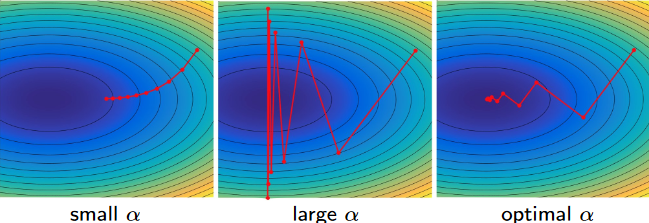
\includegraphics[width=7cm]{alpha.png}\end{center}
        L'idea generale degli algoritmi di ricerca della linea è quella di scegliere un valore diverso di $\alpha$ per 
        ogni iterazione. Data una certa iterazione, scegliamo un $\alpha$ che minimizza globalmente la funzione:
        \[\arg \min_\alpha f(x^{(t)} - \alpha \nabla f(x^{(t)})) \]
        Seguendo questo algoritmo, i passi sono ortogonali fra di loro.

    \section{Decay e momentum}
        Il parametro $\alpha$, come abbiamo già osservato, può essere \emph{adattivo} o seguire un programma.
        \subsection{Decay}
            Possiamo diminuire $\alpha$ rispetto a un parametro di decay $\rho$. Ad esempio possiamo decidere per un programma 
            lineare che modifica $\alpha$ da un certo $\alpha^{(0)}$ e che arriva a $\alpha^{(\rho)}$ con l'avanzare del tempo:
                \[\alpha^{(t+1)} = (1-\frac{t}{\rho})\alpha^{(0)} + \frac{t}{\rho}\alpha^{(\rho)} \]
            Definiamo quindi due estremi e il valore $\alpha$, con l'avanzare del tempo, passerà da un estremo all'altro in funzione del 
            parametro $\rho$. Un altro modo è quello di utilizzare un programma esponanenziale negativo, facendo diminiuire $\alpha$ 
            esponenzialmente. La velocità di decrescita dipende da $\rho$:
            \[\alpha^{(t+1)} = \alpha^{(0)}e^{-\rho t}\]
            Possiamo anche diminuire il parametro $\alpha$ iperbolicamente, sempre in funzione del parametro di decay $\rho$ e del tempo $t$:
                \[\alpha^{(t+1)} = \frac{\alpha^{(t)}}{1+\rho t}\]

        \subsection{Momentum}
            Il momentum è un meccanismo molto potente che viene dal mondo dell'ottimizzazione. Momentum aggiunge un altro 
            elemento all'equazione del gradiente:
                \[\mathbf{v}^{(t+1)} = \lambda \mathbf{v}^{(t)} - \alpha \nabla f(\mathbf{x}^{(t)})\]
                \[\mathbf{x}^{t+1} = \mathbf{x}^{t} + \mathbf{v}^{(t+1)}\]
            In cui il coefficiente $\lambda$ è detto \emph{coefficiente di momentum}. Possiamo osservare che quando $\lambda = 0$ 
            il gradiente con momentum è uguale alla normale discesa del gradiente. Per semplicità, supponiamo che 
            $\mathbf{v}^{(0)}$ è il vettore di soli zeri. Alla prima iterazione, qualsiasi sia $\lambda$, abbiamo un semplice step 
            di discesa del gradiente. Alle iterazioni successive, stiamo accumulando i gradienti sommandoli sempre, moltiplicando a 
            ogni iterazione per il coefficiente $\lambda$, pesando effettivamente sempre di più i gradienti. \\
            Possiamo osservare che la somma di due vettori è massima quando i due vettori sono \emph{colineari}. Se abbiamo deviazione 
            dalla colinearità, il gradiente inizia a decelerare, conservando comunque il momentum di prima. Questo implica che 
            fin quando stiamo scendendo lungo una direzione che rimane la stessa, i gradienti sono lineari allora 
            effettuiamo passi sempre più lunghi. Questo ci potrebbe permette di sorpassare un minimo locale facilmente, senza 
            rimanere incastrati in esso. Se invece sorpassiamo un minimo globale, ci troveremo in un punto in cui il prossimo step di 
            momentum ci dice di andare nella direzione opposta, rallentando molto il passo e tornando indietro, finché non viene 
            raggiunto il minimo. La lunghezza del passo forma una serie che converge a un certo numero ed è proporzionale a come 
            allineate sono le sequenze dei gradienti:
                \[\frac{1}{1-\lambda} \alpha ||\nabla f||\]

    \section{Accelerazioni del primo ordine}
        Possiamo scrivere la discesa del gradiente come segue:
            \[\mathbf{x}^{t+1} = \mathbf{x}^{(0)} - \alpha \sum_{i=1}^t \nabla f(\mathbf{x}^{(i)})\]
        Facendo lo stesso con il momentum invece otteniamo la seguente espressione:
            \[ \mathbf{x}^{t+1} = \alpha \sum_{i=1}^t \frac{1-\lambda^{t+1-i}}{1-\lambda} \nabla f(\mathbf{x}^{(i)})\]
        Le espressioni sono analoghe: prima pesavamo il gradiente dentro la sommatoria con un coefficiente pari a $1$, 
        mentre ora lo pesiamo da un coefficiente che dipende da $\lambda$ e che cambia a ogni $t$, ma la forma generica è sempre 
        la stessa. Quindi, in generale:
        \[\mathbf{x}^{t+1} = \mathbf{x}^{(0)} - \alpha \sum_{i=1}^t \gamma_i^t \nabla f(\mathbf{x}^{(i)})\]
        Sapendo che $\nabla f(\mathbf{x}^{(i)})$ è un vettore, invece di scalarlo per $\gamma$, possiamo 
        trasformarlo con una matrice $\Gamma$ diagonale:
        \[\mathbf{x}^{t+1} = \mathbf{x}^{(0)} - \alpha \sum_{i=1}^t \Gamma_i^t \nabla f(\mathbf{x}^{(i)})\]
        Algoritmi più sofisticati per la discesa del gradiente, come ADAM, AdaGrad, hanno una scelta di $\Gamma$ particolare.

    \section{Discesa del gradiente come tool generico}
        La discesa del gradiente è comoda per risolvere problemi non-convessi che non hanno una soluzione in forma chiusa, ma è 
        utilizzabile anche per problemi convessi come regressione lineare. La discesa del gradiente applicata alla regressione 
        lineare ci garantisce una soluzione ottima globale e non ci richiede di computare l'inversa della matrice $\mathbf{A}^T\mathbf{A}$, come 
        accade per la formula in forma chiusa. Questo vale anche per la regressione logistica, che non ha una forma chiusa ma essendo un problema convesso 
        la discesa del gradiente ci garantisce un minimo globale.


\end{document}